%\clearpage
\section{Exclusivity }
\label{sec:exclusivity}

\par With the high pileup environment in 8 TeV data it is crucial to improve
on what has been done with 7 TeV data~\cite{CMSmumu}~\cite{CMSee}~\cite{MonteNote}.
With 8 TeV data, the strategy adopted at 7 TeV of requiring a 2-track vertex
and not having another track within 3 mm is only 30\% efficient. This strategy 
 is unreliable because the vertexing algorithms can be overly enthusiastic about 
associating tracks to a vertex. As a result, originally 2-track
vertices are assigned 3 or more tracks.   

\subsection{Strategy}
\par The strategy used at 8 TeV is to demand that the lepton pair not have any tracks
other than those from the two leptons within a window in~\z0\ along 
the beamline. Tracks are taken from the trk container and required to have 
at least 1 pixel hit and at least 4 sct hits. In contrast, lepton tracks are taken 
from the lepton containers. It is therefore necessary to match the lepton tracks to two tracks from the trk container.
For a track in the trk container to be considered a match to a lepton track it is required to
be within 0.01 in $\Delta R$ and within 1 mm  in \z0, with respect to 
the beamline. The tracks in the electron or muon
containers are obtained using algorithms (GSM) different from the algorithms
used in the trk container. For this reason, a lepton track may not be matched to a track in the trk container
or may be matched to multiple tracks in the trk container. Figure~\ref{fig:trackMatching} 
shows the number of tracks from the trk container that match the leading lepton 
in the event. The distribution on the left is for matching tracks to an electron and 
that on the right is for matching tracks to muons. 
 
\begin{figure}[!h]
\centering
\begin{tabular}{c}
	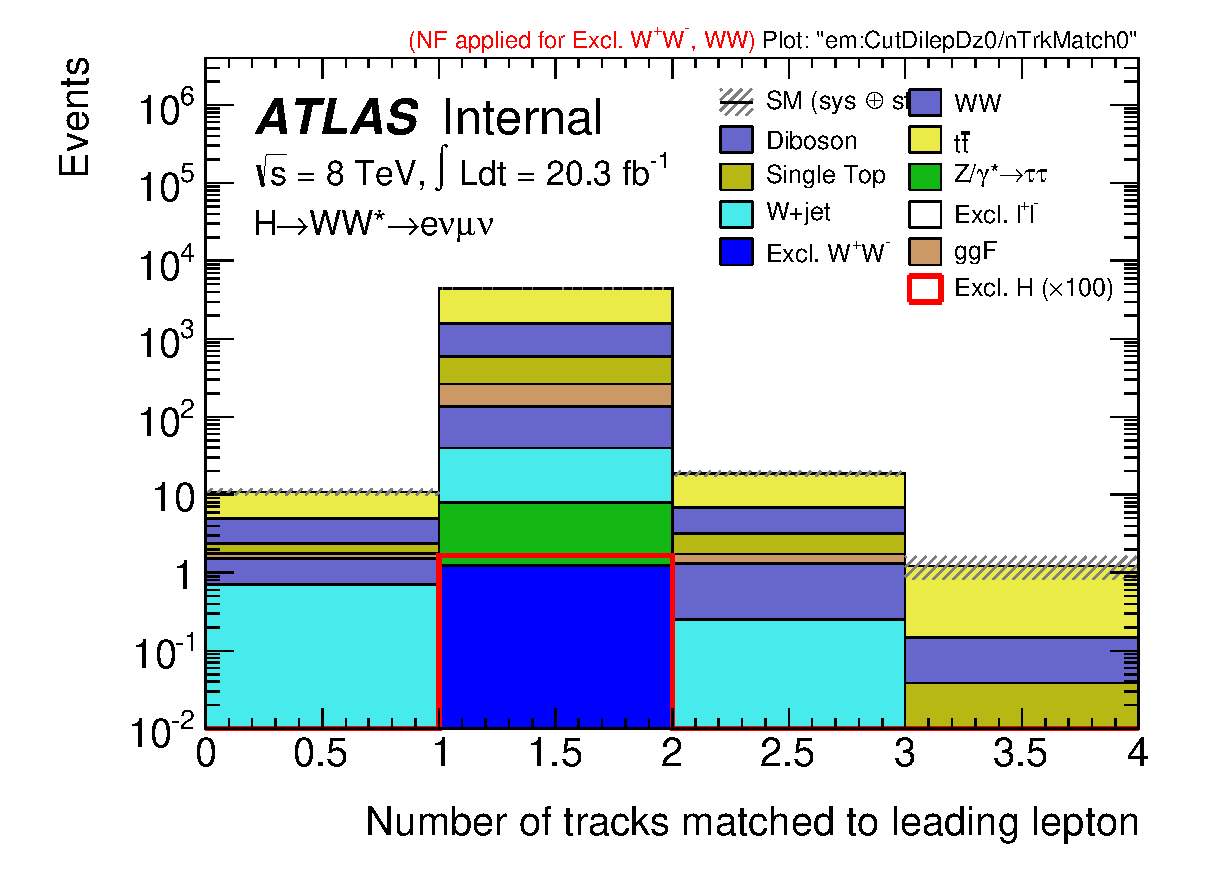
\includegraphics[width=0.5\linewidth]{em_CutDilepDz0_nTrkMatch0_mh125_log.eps}
	\includegraphics[width=0.5\linewidth]{me_CutDilepDz0_nTrkMatch0_mh125_log.eps}\\
\end{tabular}
\caption{Number of tracks from the trk container that are matched to the leading 
lepton tracks. [Left] The leading lepton is an electron. [Right] The leading lepton 
is a muon.}
\label{fig:trackMatching}
\end{figure}

\par Because electrons undergo bremsstrahlung more frequently than muons, there are more tracks 
matched to electrons than to muons. All the tracks matched to a lepton are therefore 
considered to be brehming from that lepton.

\par The exclusivity cut depends on how far in \z0\ the closest unmatched track 
is from the lepton track pair. Figure~\ref{fig:cartoon} illustrates how this is quantified. 
The two lepton tracks are first required to be within 1 mm in \z0\ to ensure that they indeed 
are from the lepton pair. The average \z0\ position computed from the individual lepton track \z0's is 
considered the dilepton vertex. The distance of the closest unmatched track $\Delta z_1$ is the 
exclusivity variable that is cut on. Figure~\ref{fig:deltaZ1} shows $\Delta z_1$  for signal and several backgrounds.
The signal is scaled by a factor of 100 to make it visible because it is heavily dominated by the backgrounds.
The $\Delta z_1$ distribution in signal and other exclusive processes 
is characterized by a tail more spread out than in inclusive processes. Several values of $\Delta z_1$ 
were tried to maximize $signal/\sqrt{background}$. Figure~\ref{fig:sOverB} shows $signal/\sqrt{background}$
for four values of $\Delta z_1$. This analysis settles on $\Delta z_1 > 1 mm$ as the optimal 
exclusivity cut.    

\begin{figure}[!h]
\centering
\begin{tabular}{c}
\includegraphics[width=0.7\linewidth]{cartoon.eps}
\end{tabular}
\caption{Illustration of the exclusivity variables.}
\label{fig:cartoon}
\end{figure}

\begin{figure}[!h]
\centering
\begin{tabular}{c}
	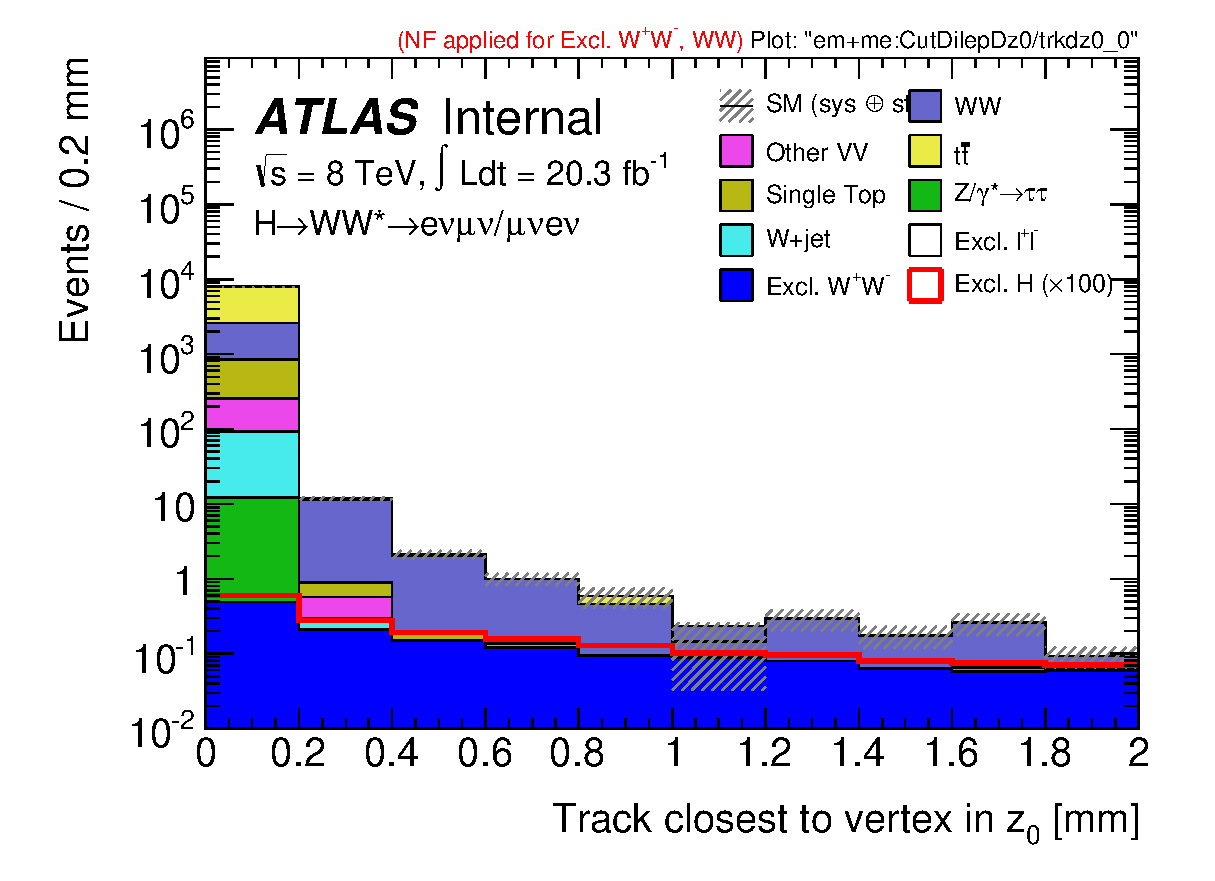
\includegraphics[width=0.5\linewidth]{trkdz0_deltaZ1.eps}
\end{tabular}
\caption{The main exclusivity variable $\Delta z_1$, which is the distance of 
the closest unmatched track to the dilepton vertex in \z0. Signal is scaled by 100. 
$\Delta z_1$ has a longer tail in exclusive processes compared to inclusive processes. 
This distrinction is exploited in this study.}
\label{fig:deltaZ1}
\end{figure}

\begin{figure}[!h]
\centering
\begin{tabular}{c}
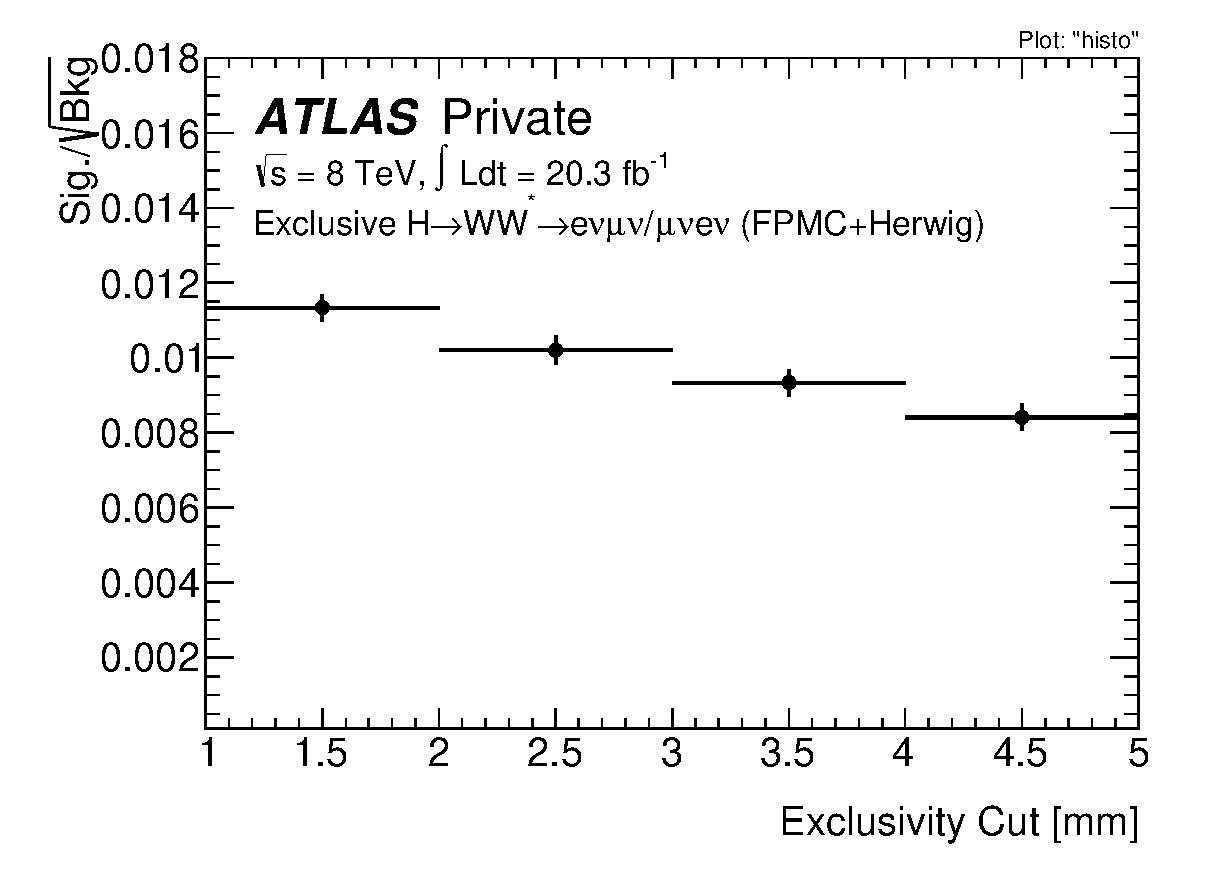
\includegraphics[width=0.7\linewidth]{emme_sOverB.eps}
\end{tabular}
\caption{$signal/\sqrt{background}$ for 4 values of $\Delta z_1$. This analysis settles 
on $\Delta z_1 > 1 mm$ as the optimal exclusivity cut.}
\label{fig:sOverB}
\end{figure}

\subsection{Performance in data}
\par A region in data that is rich in \Ztau\ events is used to validate the exclusivity selection 
criteria. This region follows the control region used in Ref.~\cite{ATLASCONF2014060} to constrain 
 \Ztau+0-jets events in the \HWW\ study. In this study we apply it to any jet multiplicity.
The selection is similar to the signal selection criteria except the following: \mll\ region is expanded to 
cover $10<\mll<80 $GeV, \ptll\ is changed to $\ptll<30 $GeV. The \dfll\ cut is also droppped. Figure~\ref{fig:ztauCR}
shows some kinematic distributions of events in this \Ztau\ region. This region achieves 
--\% purity. 

\begin{figure}[!h]
\centering
\begin{tabular}{c}
	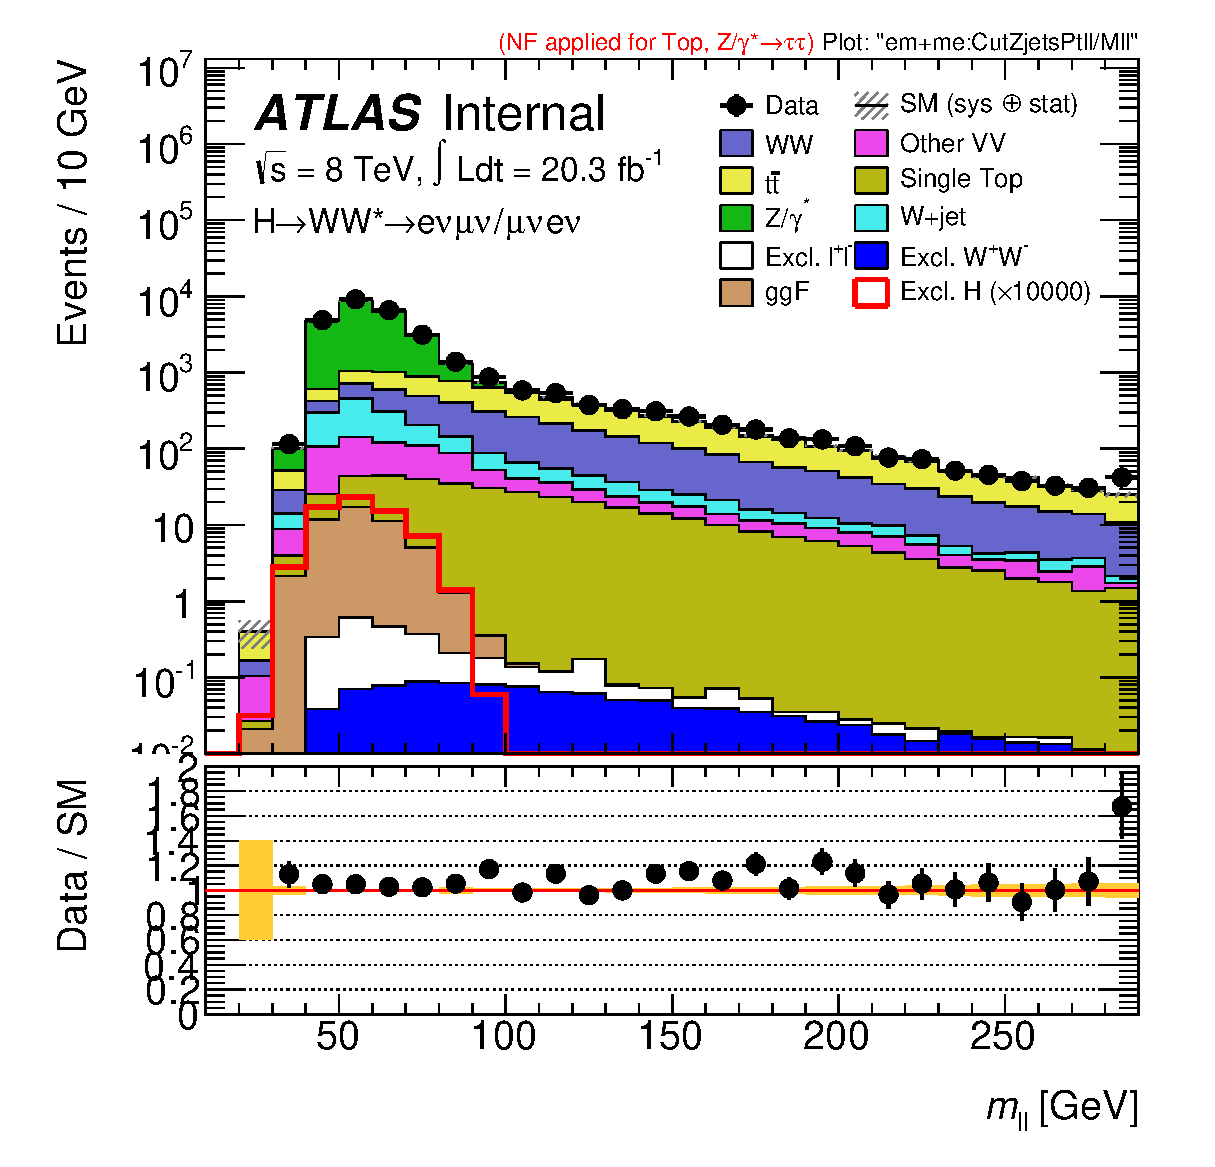
\includegraphics[width=0.5\linewidth]{emme_CutZjetsPtll_Mll_mh125_log.eps}
	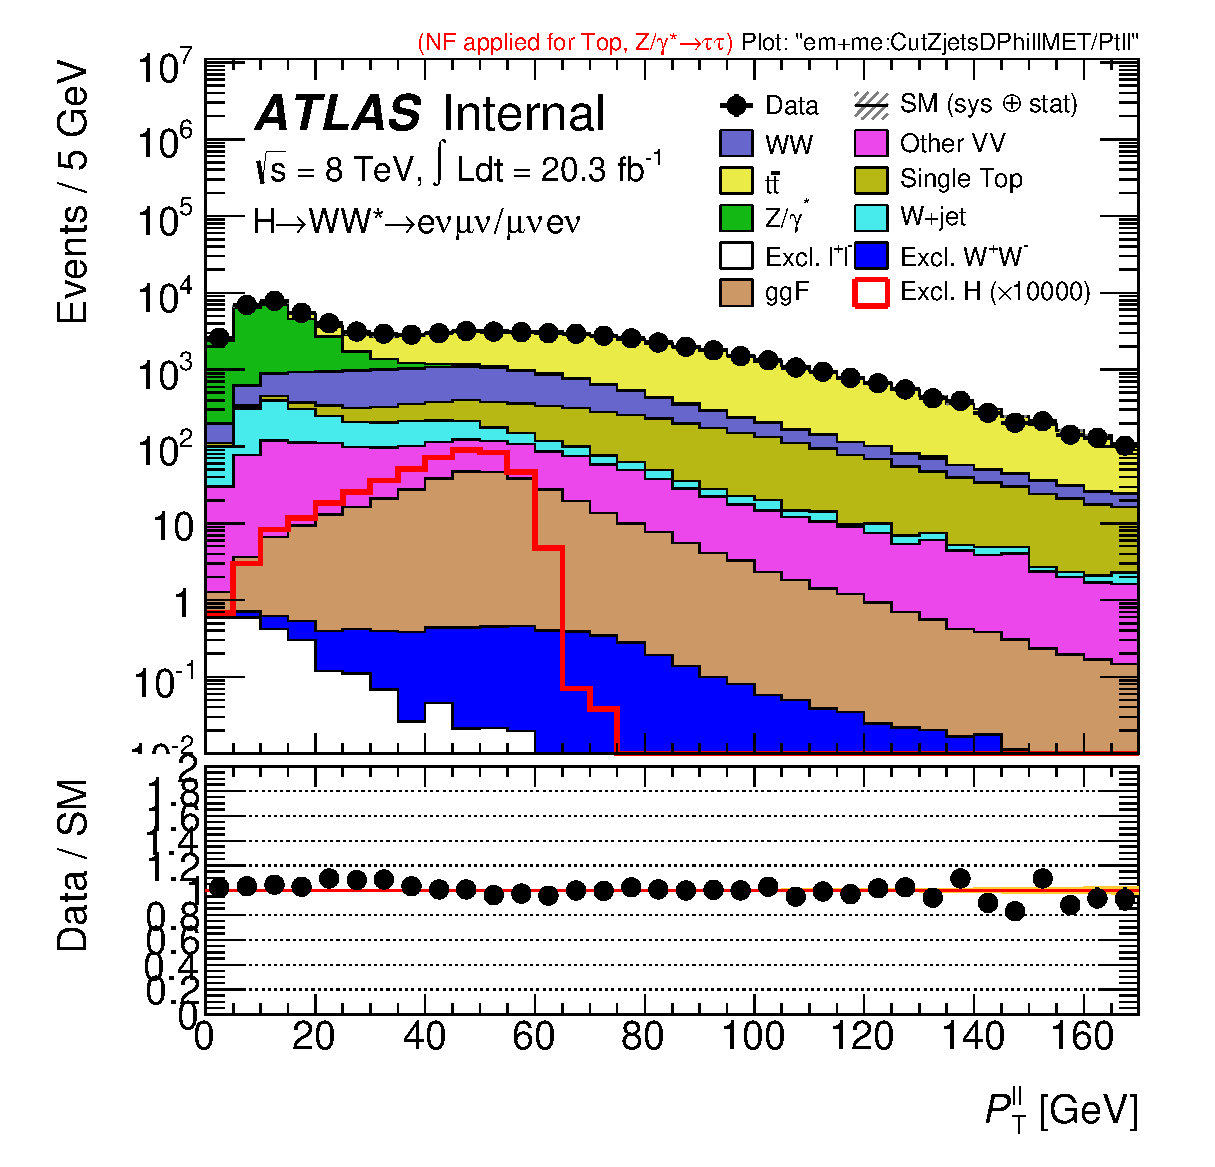
\includegraphics[width=0.5\linewidth]{emme_CutZjetsDPhillMET_Ptll_mh125_log.eps}\\
	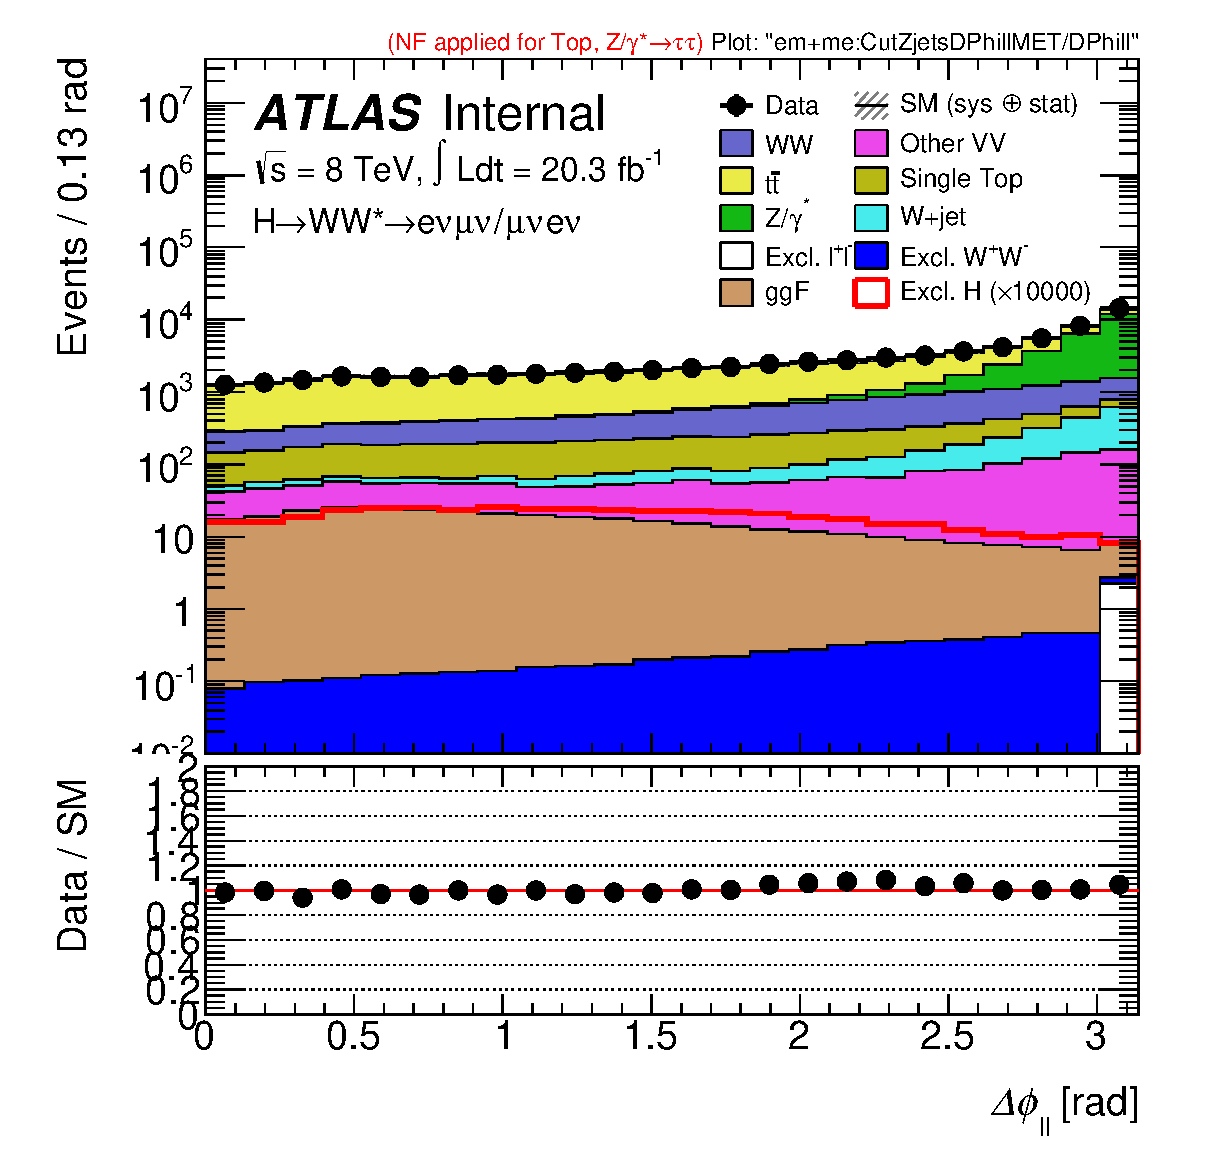
\includegraphics[width=0.5\linewidth]{emme_CutZjetsDPhillMET_DPhill_mh125_log.eps}
	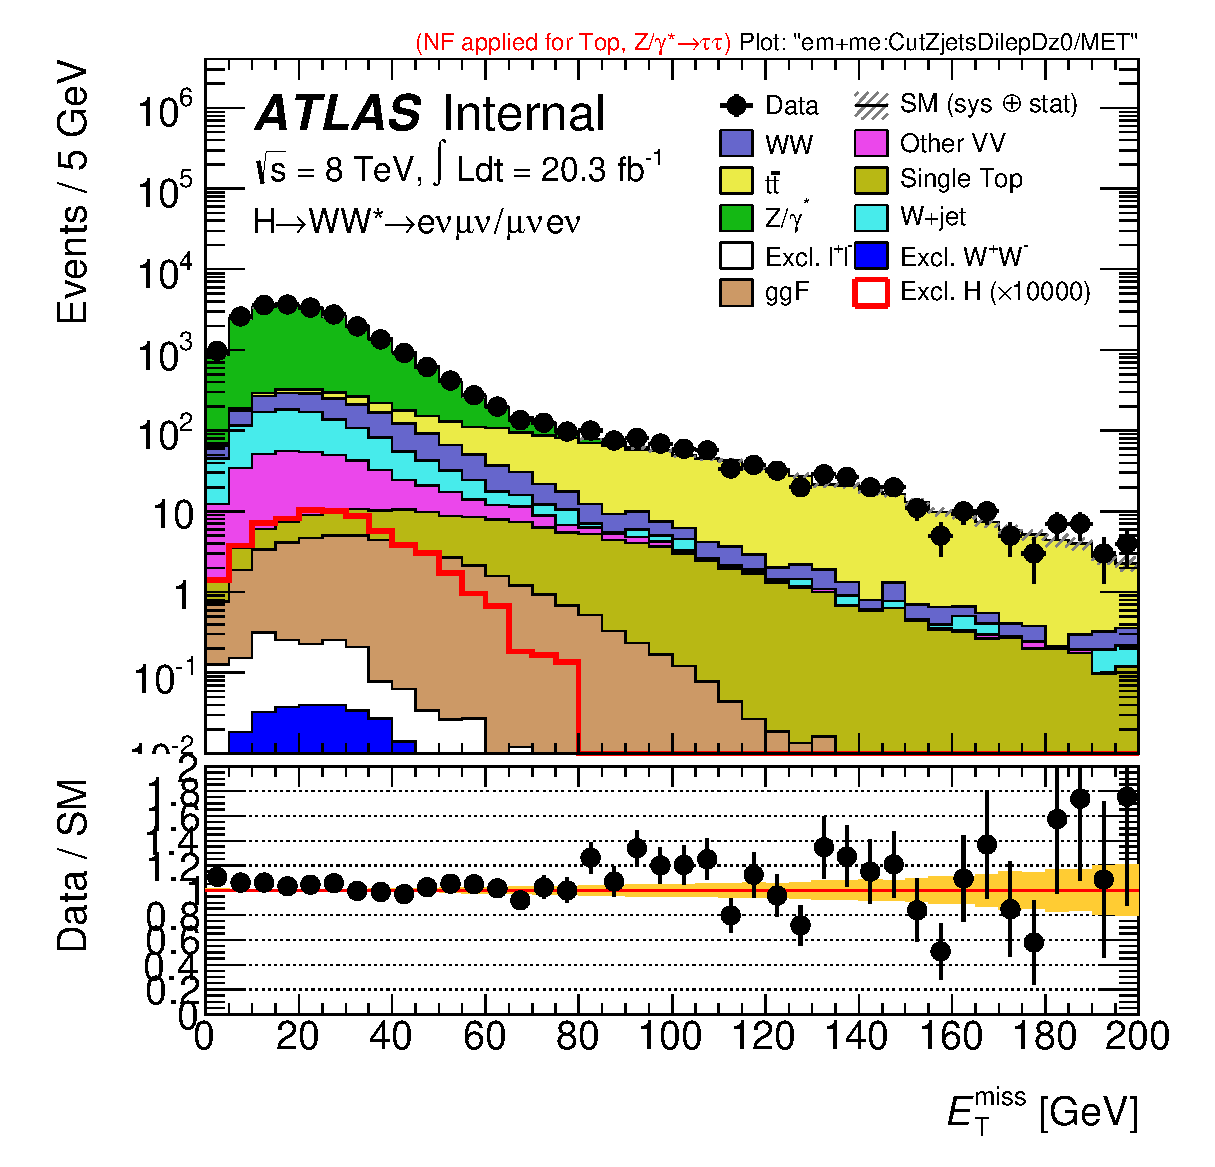
\includegraphics[width=0.5\linewidth]{emme_CutZjetsDilepDz0_MET_mh125_log.eps}\\
	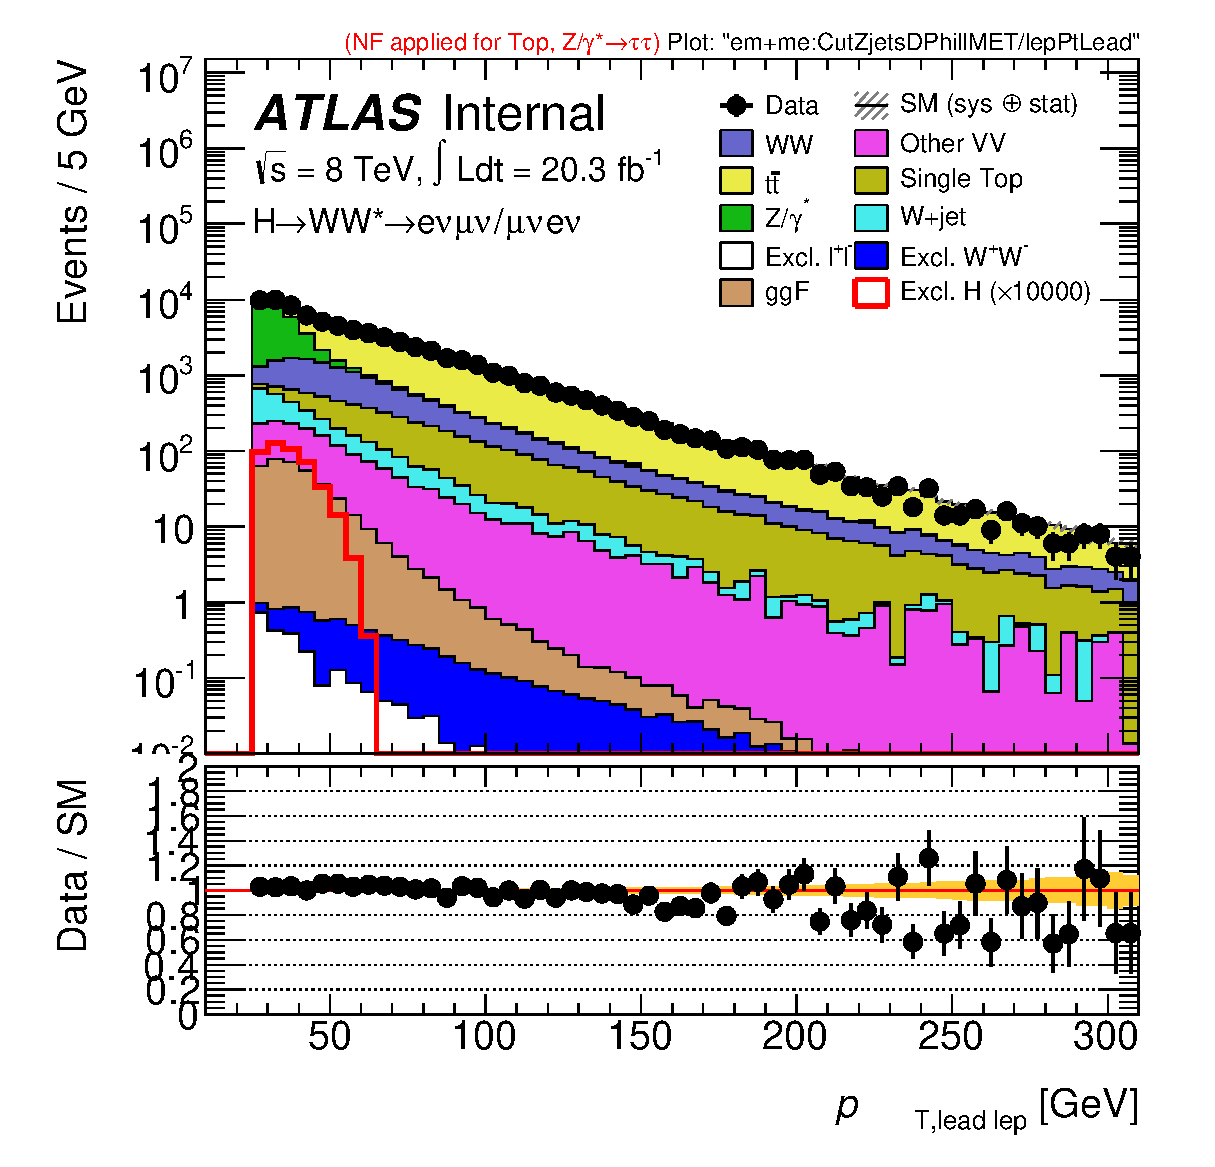
\includegraphics[width=0.5\linewidth]{emme_CutZjetsDPhillMET_lepPtLead_mh125_log.eps}
	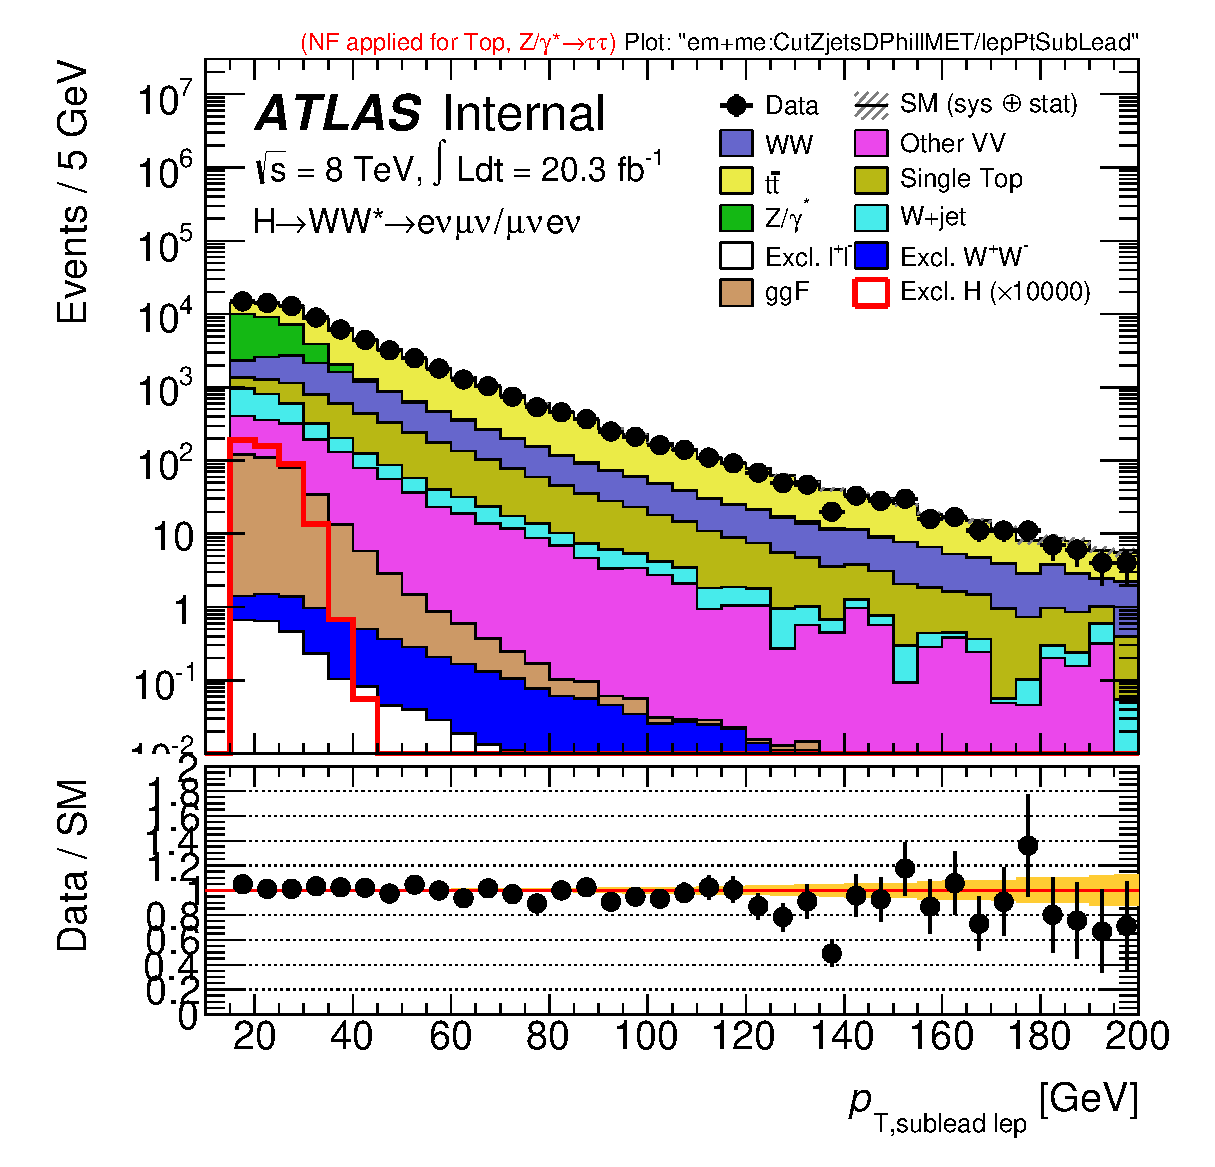
\includegraphics[width=0.5\linewidth]{emme_CutZjetsDPhillMET_lepPtSubLead_mh125_log.eps}\\
\end{tabular}
\caption{\Ztau\ CR}
\label{fig:ztauCR}
\end{figure}

\par Figure~\ref{figztauExclCR} shows exclusivity variables ... 
talk about the mismodelling factor .... 
\begin{equation}
\mbox{MC Exclusivity Correction Factor, MF} = \frac{N^{mc}_{after\ excl.}/N^{mc}_{before\ excl.}}{N^{data}_{after\ excl.}/N^{data}_{before\ excl.}}
\end{equation}
comparison between MCs ...
 
\begin{figure}[!h]
\centering
\begin{tabular}{c}
	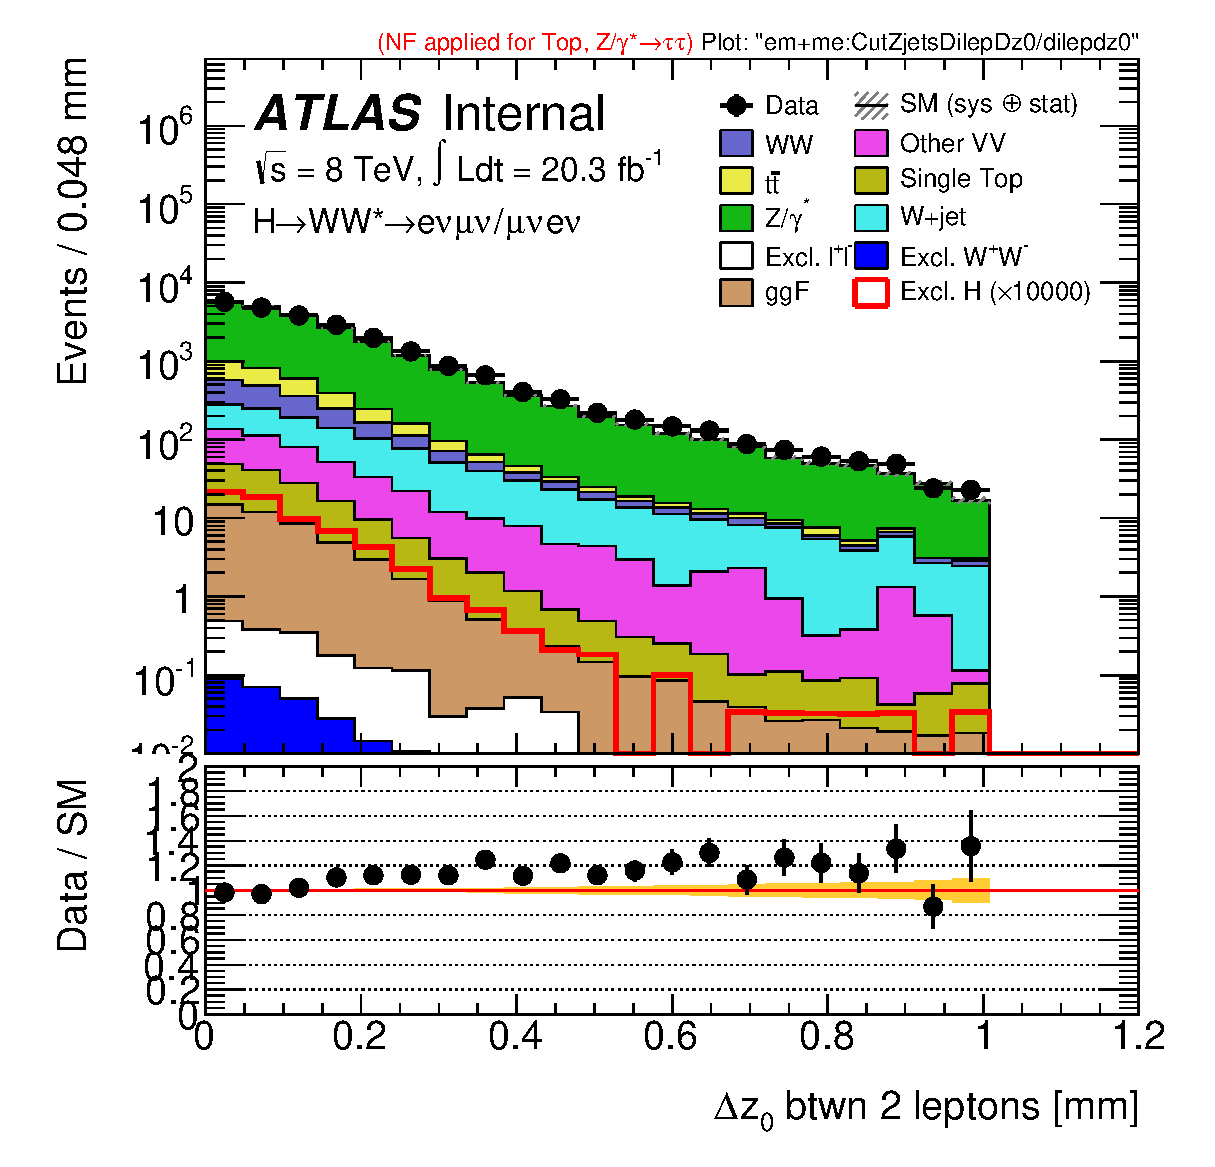
\includegraphics[width=0.5\linewidth]{emme_CutZjetsDilepDz0_dilepdz0_mh125_log.eps}
	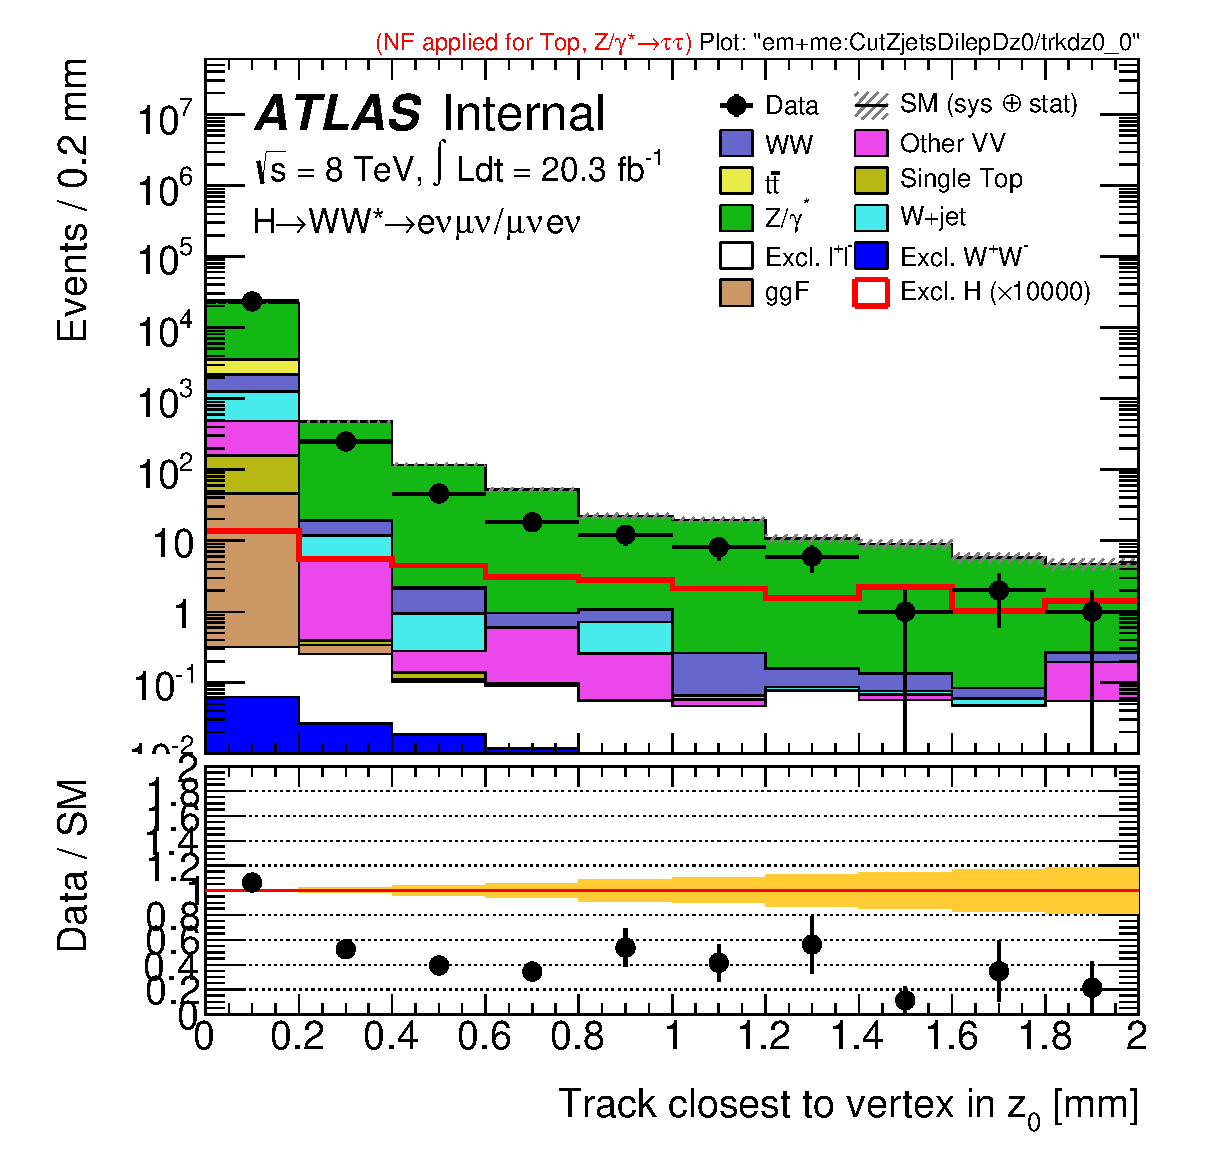
\includegraphics[width=0.5\linewidth]{emme_CutZjetsDilepDz0_trkdz0_0_mh125_log.eps}\\
\end{tabular}
\caption{Exclusivity variables in the \Ztau\ CR}
\label{fig:ztauExclCR}
\end{figure}

\begin{table}
\begin{center}
        \resizebox{0.5\textwidth}{!}{
\providecommand{\cutflowTitle}{hsg3}
\begin{tabular}{l|rr}
 & \Zmm & \Ztau   \\
\hline\hline
Sherpa &       9.23 &  \\
AlpgenPythia & 1.65 & \\
AlpgenJimmy & 4.36  & 4.72\\
PowhegPythia & 2.35 & 
\end{tabular}
}
\caption{}
\end{center}
\end{table}

\begin{figure}[!h]
\begin{tabular}{c}
	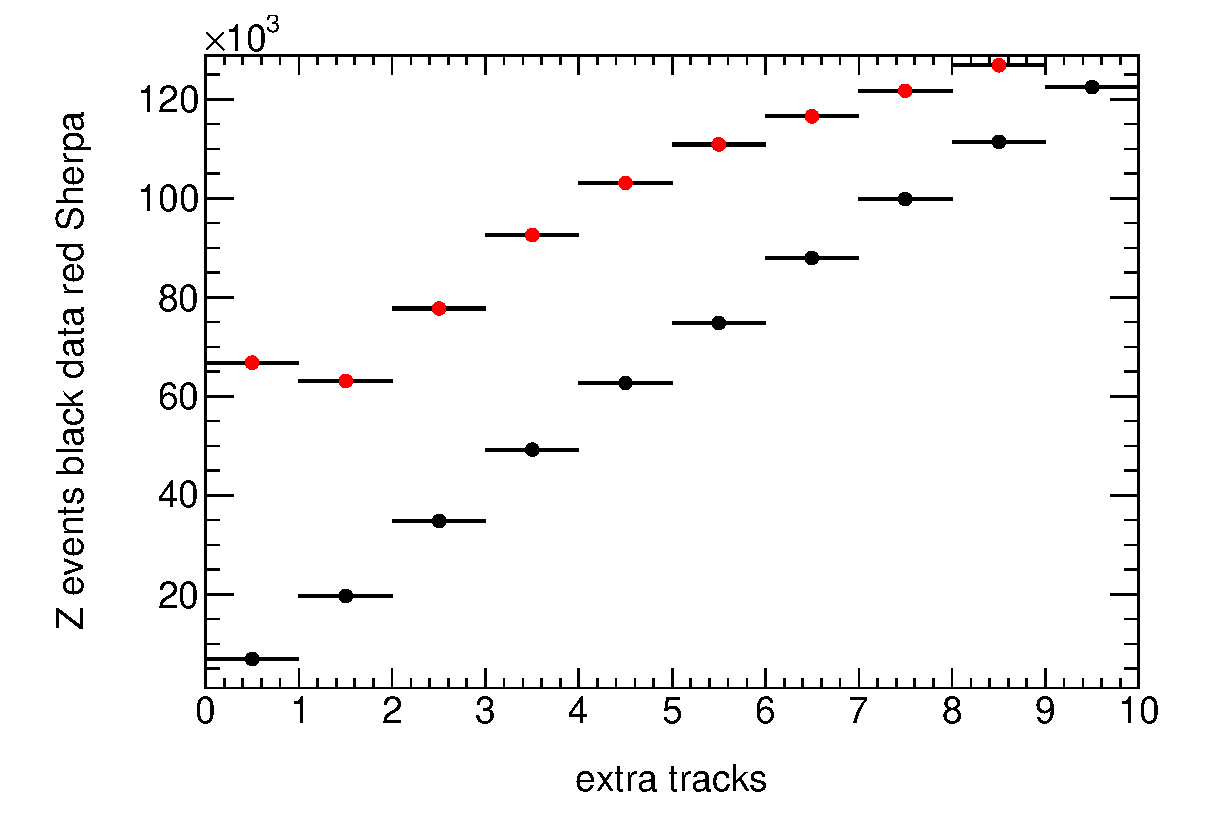
\includegraphics[width=0.5\linewidth]{extraZsherpa.eps}
	\includegraphics[width=0.5\linewidth]{extraZpowheg.eps}
\end{tabular}
\caption{Number of extra tracks within a 1.5 mm window around the di-muon vertex.}
\end{figure}
